

\chapter{Background}
\label{ch:background}

% Explain the background and theory underlying your project.
% Assume that the average reader has the same knowledge you had \emph{before} undergoing this project.
% This chapter should transfer all knowledge necessary to understand the following chapters.

% As this and the following chapters are likely longer than a few pages, consider structuring them into sections (but avoid fragmentation by overly fine-grained sectioning).
% Use the \verb|\..section{}| command family as illustrated below:

Before we look into the algorithms and theory behind reordering techniques, we first take a dive into the factorization process which produces further non-zeroes, which in this and the entire thesis' context, is called as fill-ins. Fill-ins depends only on the structure of the matrix, ie. the positions where the initial non-zero entries are placed. It may be trivial but important to note, that if some numerical arithmetic results to a zero in the factored matrix, it is usually still considered as a fill-in. 

Suppose the set of set of \textit{n} equations that are to be solved are
\begin{equation}
    Ax = b
\end{equation}
where \(A\) is a sparse matrix, \(x\) is the vector of unknowns. The sparsity, or the number of non-zero entries in \(A\) determines the fill-in of it's Cholesky factor when it is employed to solve the aforementioned set of equations. 
Suppose the Cholesky factorization of \(A\) is given by \(LL^T\), where \(L\) is a lower triangular matrix (with a positive diagonal) and \(L^T\) is the transpose of \(L\). The efficiency of solving this set of equations is dependent on the number of non-zero entries in \(L\). It has been shown (George and Liu) that we can facotr and solve the set of equations in space proportional to  \(\sum_j d_j\) and time complexity is  \(\sum_j {d_j}^2\), where \(d_j\) is the number of non-zeroes in the \(j\)th column of \(L\).
%TODO how to do sum?



\section{Elimnination Trees and Symbolic Factorization}
\label{sec:elim_tree}

The symbolic factorization phase of sparse Cholesky decomposition determines the sparsity pattern of the factor LL
L without computing numerical values. This analysis is crucial for allocating memory and understanding computational dependencies before performing the more expensive numerical factorization. The elimination tree, a fundamental data structure in sparse linear algebra, provides an elegant framework for characterizing these sparsity patterns and serves as the foundation for efficient symbolic factorization algorithms.

\subsection{Definition and Construction}

Consider a sparse symmetric positive definite matrix \(A\) of order \(n\) with its Cholesky factorization \(A = LL^T\). The elimination tree \(T(A)\) captures the structural relationships between columns of the Cholesky factor \(L\).

\begin{definition}
For each column \(j\) of the Cholesky factor \(L\), let
\[
f(j) = \min\{i > j : \ell_{ij} \neq 0\}
\]
denote the row index of the first off-diagonal nonzero entry. If column \(j\) contains no off-diagonal nonzeros, we set \(f(j) = j\).
\end{definition}

The elimination tree \(T(A)\) is constructed by defining \(f(j)\) as the parent of node \(j\) for each \(j = 1, 2, \ldots, n-1\). Node \(n\) serves as the root since \(f(n) = n\).

\begin{theorem}
The elimination tree \(T(A)\) is a spanning tree of the filled graph \(G^+(A)\) satisfying:
\[
\text{parent}[j] = \min\{i > j : \ell_{ij} \neq 0\}
\]
\end{theorem}

\subsection{Fundamental Properties}

The elimination tree reveals the inherent structure of sparse Cholesky factorization through several key properties.

\begin{theorem}[Path Characterization of Fill-in]
An entry \(\ell_{ij} \neq 0\) exists in the Cholesky factor if and only if node \(i\) is an ancestor of node \(j\) in the elimination tree \(T(A)\).
\end{theorem}

This theorem provides a direct correspondence between nonzero entries in \(L\) and ancestor-descendant relationships in the tree, making the elimination tree a complete characterization of the factor's sparsity pattern.

\begin{theorem}[Subtree Independence]
Let \(T[x_i]\) and \(T[x_j]\) be two disjoint subtrees of \(T(A)\). Then \(\ell_{st} = 0\) for any \(x_s \in T[x_i]\) and \(x_t \in T[x_j]\).
\end{theorem}

This independence property reveals the potential parallelism available in sparse factorization, as computations involving disjoint subtrees can proceed without interference.

\subsection{Sparsity Pattern Characterization}

\paragraph{Row Structure Analysis}

The elimination tree enables precise characterization of row sparsity patterns through the concept of row subtrees.

\begin{theorem}[Row Structure]
Let \(i > j > k\). The entry \(\ell_{ij} \neq 0\) if and only if node \(x_j\) is an ancestor of some node \(x_k\) in the elimination tree where \(a_{ik} \neq 0\).
\end{theorem}

\begin{definition}[Row Subtree]
For row \(i\) of \(L\), the row subtree \(T_r[x_i]\) is defined as:
\[
T_r[x_i] = \{x_j : \ell_{ij} \neq 0,\, j \leq i\}
\]
\end{definition}

The row subtree can be constructed by identifying all nodes \(x_k\) where \(a_{ik} \neq 0\) and including all ancestors of these nodes up to (but not including) node \(i\) itself. Equivalently, \(T_r[x_i]\) is obtained from the elimination tree \(T[x_i]\) by pruning at the leaves corresponding to nonzeros in the original matrix \(A\).

\paragraph{Column Structure Analysis}

The dual perspective considers column sparsity patterns:

\begin{theorem}[Column Structure]
The structure of column \(j\) of \(L\) is given by:
\[
\{x_i : \ell_{ij} \neq 0,\, i \geq j\} = \text{Adj}_{G(A)}(T[x_j]) \cup \{x_j\}
\]
where
\[
\text{Adj}_{G(A)}(S) = \{x \notin S : x \in \text{Adj}_{G(A)}(v) \text{ for some } v \in S\}
\]
denotes the adjacency of set \(S\) in the original graph \(G(A)\).
\end{theorem}

This characterization shows that the nonzeros in column \(j\) of \(L\) consist of node \(j\) itself plus all nodes adjacent (in the original graph) to any node in the subtree rooted at \(j\).

\section{Sequential Algorithms for Elimination Tree and Symbolic Factorization}

\subsection{Elimination Tree Construction}

The elimination tree can be computed efficiently using a union-find data structure that tracks connected components during symbolic elimination. The following algorithm constructs the elimination tree parent array:

% \begin{algorithm}[H]
% \caption{Sequential Elimination Tree Construction}
% \begin{algorithmic}[1]
% \REQUIRE Sparse matrix $A$ of order $n$
% \ENSURE Elimination tree parent array $\text{parent}[1..n]$
% \FOR{$i = 1$ \TO $n$}
%     \STATE $\text{makeset}(i)$
%     \STATE $\text{parent}[i] \gets 0$
%     \FOR{each $k < i$ where $a_{ik} \neq 0$}
%         \STATE $u \gets \text{find}(k)$
%         \IF{$\text{parent}[u] = 0$ and $u \neq i$}
%             \STATE $\text{parent}[u] \gets i$
%             \STATE $\text{link}(i, u)$
%         \ENDIF
%     \ENDFOR
% \ENDFOR

% \end{algorithm}

Using path compression and union-by-rank heuristics, this algorithm achieves complexity $O(m\alpha(m,n))$, where $m$ is the number of nonzeros in $A$ and $\alpha$ is the inverse Ackermann function.

\subsection{Symbolic Factorization}

Once the elimination tree is constructed, the sparsity pattern of $L$ can be computed by traversing row subtrees:

% \begin{algorithm}[H]
% \caption{Row-wise Symbolic Factorization}
% \begin{algorithmic}[1]
% \REQUIRE Matrix $A$, elimination tree $T$
% \ENSURE Sparsity pattern $\text{Struct}[L, i]$ for each row $i$
% \FOR{$i = 1$ \TO $n$}
%     \STATE $\text{marker}[x_i] \gets i$
%     \STATE $\text{Struct}[L, i] \gets \{i\}$ \COMMENT{Include diagonal}
%     \FOR{each $k < i$ where $a_{ik} \neq 0$}
%         \STATE $j \gets k$
%         \WHILE{$\text{marker}[x_j] \neq i$}
%             \STATE $\text{Struct}[L, i] \gets \text{Struct}[L, i] \cup \{j\}$
%             \STATE $\text{marker}[x_j] \gets i$
%             \STATE $j \gets \text{parent}[j]$
%         \ENDWHILE
%     \ENDFOR
% \ENDFOR
% \end{algorithmic}
% \end{algorithm}

The marker array prevents redundant traversals. This algorithm runs in $O(\text{nnz}(L))$ time, making it output-sensitive.

\subsection{Efficient Row and Column Counting}

For memory allocation, it is often sufficient to compute only the number of nonzeros in each row and column:

% \begin{algorithm}[H]
% \caption{Row and Column Count}
% \begin{algorithmic}[1]
% \REQUIRE Matrix $A$, elimination tree $T$
% \ENSURE Row counts $\text{rc}[]$, column counts $\text{cc}[]$
% \FOR{$j = 1$ \TO $n$}
%     \STATE $\text{cc}[j] \gets 1$
% \ENDFOR
% \FOR{$i = 1$ \TO $n$}
%     \STATE $\text{rc}[i] \gets 1$
%     \STATE $\text{marker}[x_i] \gets i$
%     \FOR{each $k < i$ where $a_{ik} \neq 0$}
%         \STATE $j \gets k$
%         \WHILE{$\text{marker}[x_j] \neq i$}
%             \STATE $\text{rc}[i] \gets \text{rc}[i] + 1$
%             \STATE $\text{cc}[j] \gets \text{cc}[j] + 1$
%             \STATE $\text{marker}[x_j] \gets i$
%             \STATE $j \gets \text{parent}[j]$
%         \ENDWHILE
%     \ENDFOR
% \ENDFOR
% \end{algorithmic}
% \end{algorithm}

Gilbert, Ng, and Peyton developed a more sophisticated approach that computes these counts in $O(m\alpha(m,n))$ time by exploiting postorder traversals of the elimination tree and least common ancestor computations, avoiding explicit traversal of row subtrees.


% \subsection{First subsection}

% \subsection{Second subsection}

\section{Heuristics classification}
\label{sec:heuristics}

There are several heuristics that have been proposed to reduce the fill-in developed over the years. These heuristics can be broadly classified in the following categories: Bandwidth minimization, minimum degree (and it's variants), nested dissection, banded structure methods using hypergraphs, and recently, machine learning approaches. 

\subsection{Bandwidth Minimization}

Bandwidth minimization refers to the problem of permuting the rows and columns of a matrix such that the non-zero entries are as close to the diagonal as possible.  Gaussian elimination can be performed in $O(nb^2)$ time on matrices of dimension $n$ and bandwidth $b$, which is faster than the forward $O(n^3)$ algorithm when $b$ is smaller than $n$ (Lim A. et al., 2006a).  Additionally, this problem is NP-complete, but several heuristics have been developed to approximate the optimal solution.

The Cuthill-McKee algorithm employs breadth-first search to reduce matrix bandwidth by generating level structures. However, it has computational limitations and may not achieve optimal bandwidth reduction. The Reverse Cuthill-McKee algorithm addresses these issues by reversing the ordering, while the GPS algorithm by Gibbs et al. provides an alternative level structure approach.

We take a look at the reverse Cuthill-McKee algorithm, which is still widely used in practice. 

[write the pseudocode here]

\subsection{Minimum Degree}

The minimum degree algorithm determines the order in which to eliminate variables (or pivot) during Gaussian elimination to minimize fill-in (creation of new non-zero entries) in sparse matrices. At each step, it chooses the node with the minimum degree (fewest connections) for elimination.

The minimum degree algorithm operates on the adjacency graph of the sparse matrix. It begins by initializing the graph, where each vertex represents a variable. At each iteration, the algorithm selects the vertex with the smallest degree (i.e., the fewest neighbors), which corresponds to the variable whose elimination is expected to introduce the least fill-in. Upon elimination, the chosen vertex is removed from the graph, and all its neighbors are connected to each other, forming a clique to preserve the matrix structure. The degrees of the affected vertices are then updated to reflect the new connections. This process is repeated until all vertices have been eliminated. The resulting elimination order directly determines the pivot sequence used during matrix factorization.

(placeholder for general algorithm) \\

Variants of the minimum degree algorithm include:

\begin{enumerate}
    \item Multiple Minimum Degree (MMD)

    When multiple nodes have the same minimum degree, uses additional tie-breaking rules. Often selects based on secondary criteria like external degree or node numbering.

    \item Approximate Minimum Degree (AMD)

    Uses approximations to avoid expensive exact degree calculations. Employs concepts like "supervariables" and "element absorption". Much faster than exact minimum degree while maintaining similar fill-in quality.

    \item Constrained Minimum Degree

    Incorporates additional constraints (like maintaining bandwidth). Balances minimum degree objective with other structural requirements.

\end{enumerate}

\subsection{Nested Dissection}

Nested dissection is a divide and conquer heuristic for the solution of sparse symmetric systems of linear equations based on graph partitioning. Nested dissection can be viewed as a recursive divide-and-conquer algorithm on an undirected graph; it uses separators in the graph, which are small sets of vertices whose removal divides the graph approximately in half  \cite{lipton_generalized_1979}.

\begin{figure}[htbp]
    \centering
    \begin{subfigure}[b]{0.45\textwidth}
        \centering
        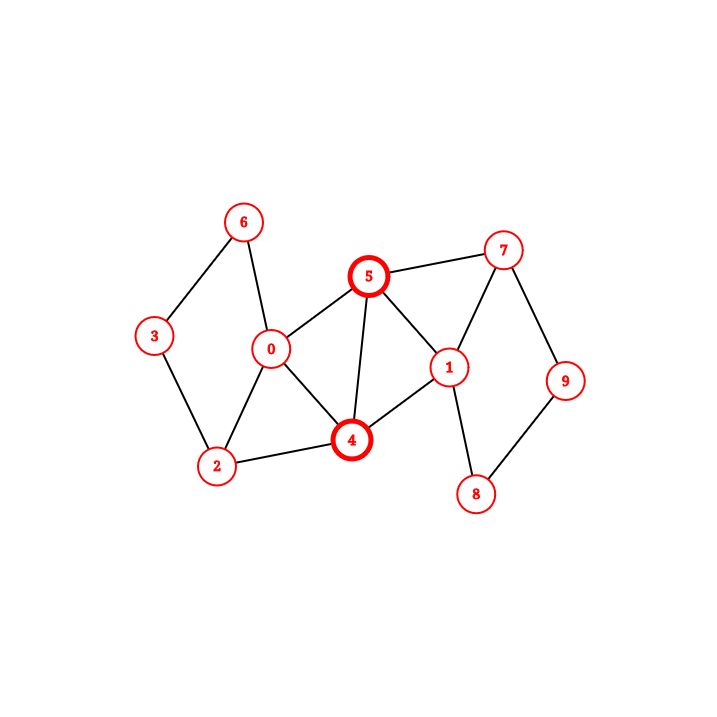
\includegraphics[width=\textwidth]{fig/background/nd-1.png}
        \caption{Original graph before separator identification}
        \label{fig:nd-original}
    \end{subfigure}
    \hfill
    \begin{subfigure}[b]{0.45\textwidth}
        \centering
        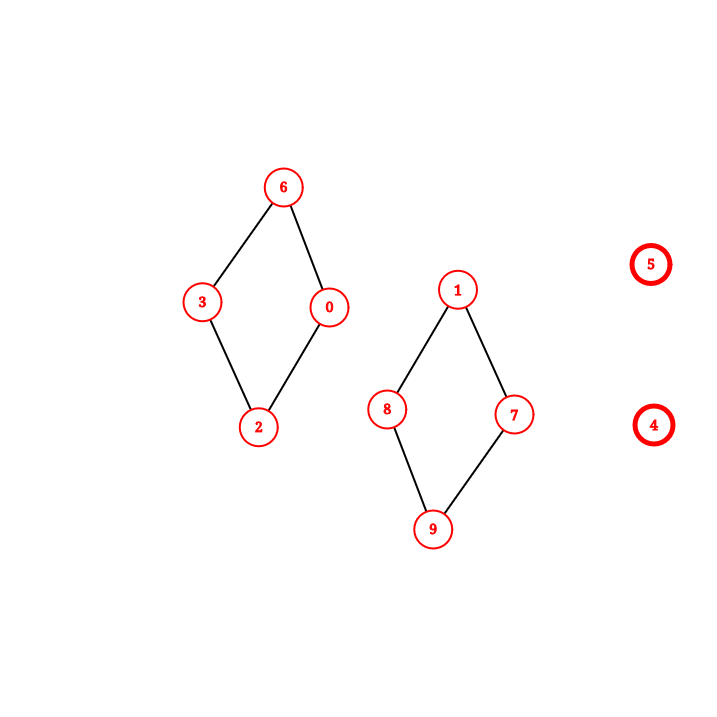
\includegraphics[width=\textwidth]{fig/background/nd-2.png}
        \caption{Graph after separator removal showing partitioned subgraphs}
        \label{fig:nd-separated}
    \end{subfigure}
    \caption{Separator identification process. The separator vertices divide the graph into approximately equal subgraphs}
    \label{fig:nested-dissection}
\end{figure}

Nested dissection consists of the following steps: Form an undirected graph in which the vertices represent rows and columns of the system of linear equations, and an edge represents a nonzero entry in the sparse matrix representing the system. Recursively partition the graph into subgraphs using separators, small subsets of vertices the removal of which allows the graph to be partitioned into subgraphs with at most a constant fraction of the number of vertices. Perform Cholesky decomposition (a variant of Gaussian elimination for symmetric matrices), ordering the elimination of the variables by the recursive structure of the partition: each of the two subgraphs formed by removing the separator is eliminated first, and then the separator vertices are eliminated \cite{george_nested_1973}. 

All the sequential algorithms for determining the elimination ordering of a graph G can be described by the following general algorithm: Generate the tree of separators for G and perform a tree traversal on the separator tree to order the vertices, where this traversal must visit a node before any of its parents.


